\documentclass[12pt]{article}
\usepackage[margin=0.7in]{geometry} 		% defines page margin
\usepackage{knitting} 				% defines \chart and \textknit
\usepackage{titling} 				% title page
\usepackage{graphicx,xspace, scrextend}	% defines space control stuff
\usepackage{tabularx, array, colortbl}	% defines tables
\usepackage{multicol} 				% defines columns
\usepackage{multirow} 				% defines multirows, combined cells in tables
\usepackage{framed} 				% defines boxes for notes and written directions
\usepackage[x11names]{xcolor} 		% extends color library
\usepackage{hyperref, wrapfig}				% hyperlinks
\hypersetup{
    colorlinks=true,
    linkcolor=blue,
    filecolor=magenta,      
    urlcolor=blue,
}

\pdfmapfile{+knitfont.map}

% font selection
\usepackage{palatino, moresize, sectsty}
\allsectionsfont{\sffamily}

% PICK AND CHOOSE COMMANDS BASED ON NEEDS

\renewcommand{\arraystretch}{2} % compresses tables for pattern keys

\newcolumntype{L}[1]{>{\leftalign\arraybackslash}p{#1}}
\newcolumntype{C}[1]{>{\centering\arraybackslash}p{#1}}

% length parameters
\setlength{\parindent}{0pt} % disables indentation for paragraphs
\setlength{\columnsep}{0.7cm} % column separation in multicol environment

% color parameters
\colorlet{framecolor}{black}
\colorlet{shadecolor}{LemonChiffon1}
\colorlet{highlight}{yellow}

% custom commands
\newcommand{\comment}[1]{} % allows for multiline comments that LaTeX will ignore

\newcommand{\vocab}[1]{\emph{\textbf{#1}}} % format for highlighting definitions of stitches, vocabulary terms
\newcommand{\rowDir}[1]{\textbf{#1:}} % indent for written instructions within paragraphs

\renewcommand{\repeat}[1]{\textbf{[#1]}} % format for written repeats, bold with *[ stitches ]*
\newcommand{\repmark}{\textbf{*}}
\newcommand{\longrepeat}[1]{\textbf{\repmark}~ #1, repeat from \repmark}%\textbf{*}}
\newcommand{\x}{$\times$}			% times symbol but shorthand
\newcommand{\setrepeat}[2]{\textbf{[#1]}\x{#2}}		% format for repeats with set number of repetitions, bold with [ stitches ]

\newcommand{\blank}{\underline{\hspace{2em}} } % written instructions, fill-in-the-blank box
\newcommand{\highlighted}[1]{\colorbox{highlight}{#1}} % written instructions, highlight particular text
\newcommand{\adjustment}[1]{\emph{#1}} % formatting for adjustment instructions

% stitch count commands
\newcommand{\increase}[1]{(\emph{+#1 
	\ifnum#1=1{st}\else{sts}\fi})}
\newcommand{\decrease}[1]{(\emph{$-$#1
	\ifnum#1=1{st}\else{sts}\fi})}
\newcommand{\stitchcount}[1]{(\emph{#1 sts})}

% marker instructions
\renewcommand{\pm}[1]{\emph{pm #1}} % place stitch marker
\newcommand{\sm}{\emph{sm}} % slip marker
\renewcommand{\rm}[1]{\emph{rm #1}} % remove stitch marker

% thick horizontal line
\makeatletter \newcommand{\thickhline}{
    \noalign {\ifnum 0=`}\fi \hrule height 1.5pt
    \futurelet \reserved@a \@xhline
}
\makeatother

% custom environments
\newenvironment{frnote}
    {% framed environment for pattern notes
    	\setlength{\FrameRule}{1.5pt}
    	\def\FrameCommand{\fboxrule=\FrameRule\fboxsep=\FrameSep \fcolorbox{framecolor}{shadecolor}}
    	\MakeFramed {\FrameRestore}}
    {\setlength{\FrameRule}{1pt}
	\endMakeFramed}

\newenvironment{frdirection}
    {% framed environment for written directions
	\def\FrameCommand{\fboxrule=\FrameRule\fboxsep=\FrameSep \fbox}
   	\MakeFramed {\advance\hsize-\width \FrameRestore}
    	\addmargin[2em]{0pt}}
    {\endaddmargin
	\endMakeFramed}

\newenvironment{unframed}
    {% unframed environment for written directions
	\begin{addmargin}[2em]{0pt}
	\setlength{\parindent}{-2em}}
    {%\vspace{1em}
	\setlength{\parindent}{0em}
	\end{addmargin}}

\title{Kickshaws} % pattern name here
\author{Shanel Wu (Piper Nell)}

\begin{document}

%%%%%%%%%%%%%%%%%%%%%%%%%%%%%%%%%%%%%%%%%%%%%%%%%%
% TITLE PAGE 
\begin{titlingpage}

% COVER PHOTO
% uncommend line below if you want a background fill image
% \ThisLRCornerWallPaper{1.0}{image.jpg} 

{\fontfamily{qag}\selectfont
\HUGE\textbf{\thetitle}
\hspace{2em} \hfill % adjust this space or use \hfill
\normalsize\theauthor
}

~\\
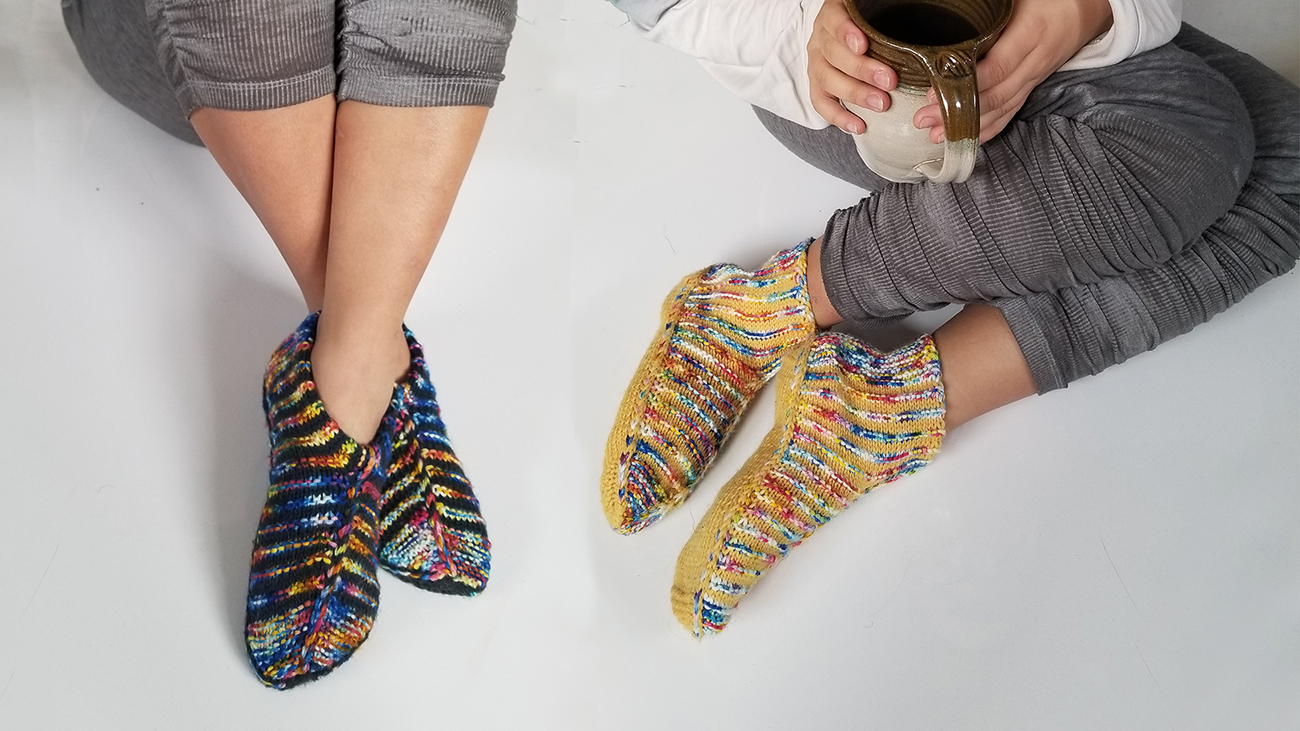
\includegraphics[width=\linewidth]{./photos/smallVersions/bothMe_LANDSCAPE_200dpi.jpg}

\begin{multicols}{2}
\small

% Cute description here
``Art thou good at these \emph{kickshawses}!” wrote Shakespeare, a slang term from him for something frivolously fancy and fun. These slippers will be a fun project, and make you feel fancy during the colder seasons, but they are certainly not frivolous! Warm and practical, the three-part construction allows you to custom-fit the slippers. \vspace{-1em}

\subsection*{Sizing: XS (S, M, L)}
Sizing, fit, and dimensions details on next page.

\subsection*{Gauge: 5.5 sts = 1"/2.5cm}

22 sts $\times$ 30 rows = 4"/10cm in stockinette.

22 sts $\times$ 44 rows = 4"/10cm in unstretched garter stitch. All gauges given without blocking.

\subsection*{Yarn Requirements}

Worsted weight wool yarn in two contrasting colors, MC and CC.

% yardage, number of colors, etc.
\rowDir{MC} 25 (90, 160, 210) yds / 25 (85, 150, 200) m  % yards and meters

\rowDir{CC} 25 (80, 130, 180) yds / 25 (75, 120, 170) m  % yards and meters

~\vfill
\columnbreak
\scriptsize
% also include: sample yarn, other yarn suggestions
\emph{Sample: MC - Kelbourne Woolens Germantown (220yds/100g, 100\% wool) in Black (left) and Goldenrod (right); CC - Knitted Wit Merino Worsted (200yds/113g, 100\% Merino) in ``Hand in Hand"}

\small
% sample measurements, gauge, notes on ease, etc.
\subsection*{Tools}

\begin{itemize}
\item US4/3.5mm (or size needed to obtain tight gauge) in any style
\item tapestry needle
\end{itemize}

\subsection*{Techniques}

This pattern is suitable for an advanced beginner. % DIFFICULTY LEVEL
Prior to knitting this pattern, you should be familiar with casting on, knitting, purling, k2tog, kfb, and slipping stitches. % PREREQUISITE TECHNIQUES
Technical support is provided for striping yarns and picking up stitches. Guidelines are also provided for some suggested modifications after the pattern instructions.
For a complete list of stitches used, see Pattern Key.

% discuss any special techniques and tutorials included

~\vfill
\newpage

%\subsection*{Schematic}

\subsection*{Finished Dimensions and Fit}

\textbf{Sizes} roughly correspond to baby (child/adult narrow, adult medium, adult large/wide) feet to fit:

\begin{unframed}
Euro 18-24 (25-32, 33-43, 44,49) \\
US children's 0-3.5 (4-13.5, -, -) \\
US women's - ( -, 5-11.5, 12+) \\
US men's - ( -, 3.5-10, 10.5, 15)
\end{unframed}

~\\
\rowDir{Foot Width} 2 (3, 4, 5)" / 5 (7.5, 10, 12.5) cm

\rowDir{Foot length} 4 (7, 10, 13)" / 10 (17.5, 25, 32.5, 37.5) cm as written in instructions. \emph{Can be adjusted between 3-5 (5-8, 8-11, 11-13)" / 7.5-12.5 (12.5-20, 20-27.5, 27.5-32.5) cm. \\~\\ Adjusting length will affect yardage requirements.}

~\\
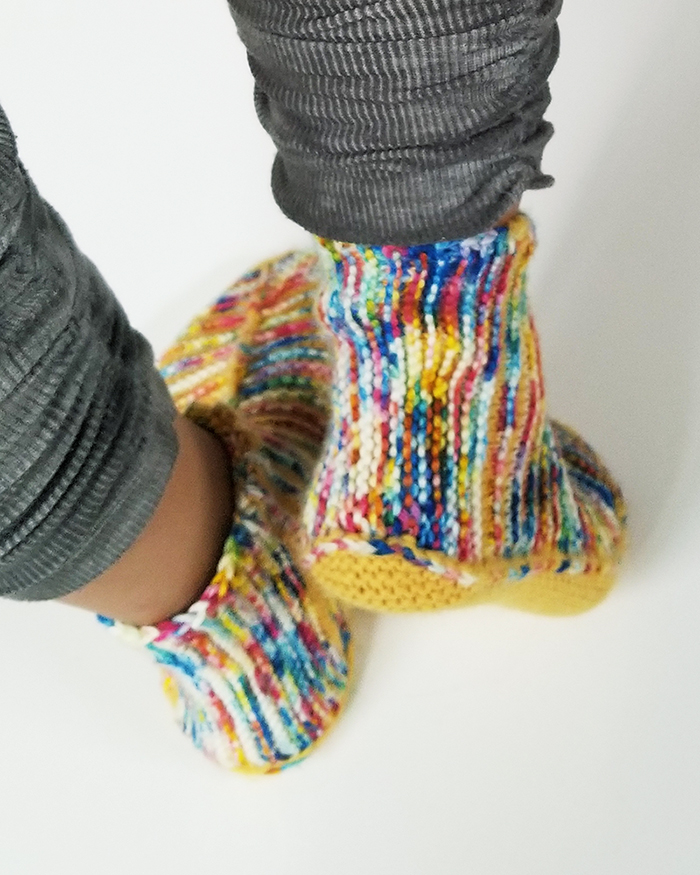
\includegraphics[width=\linewidth]{./photos/smallVersions/yellow_backs_200dpi.jpg}

\vfill
~\\

\columnbreak

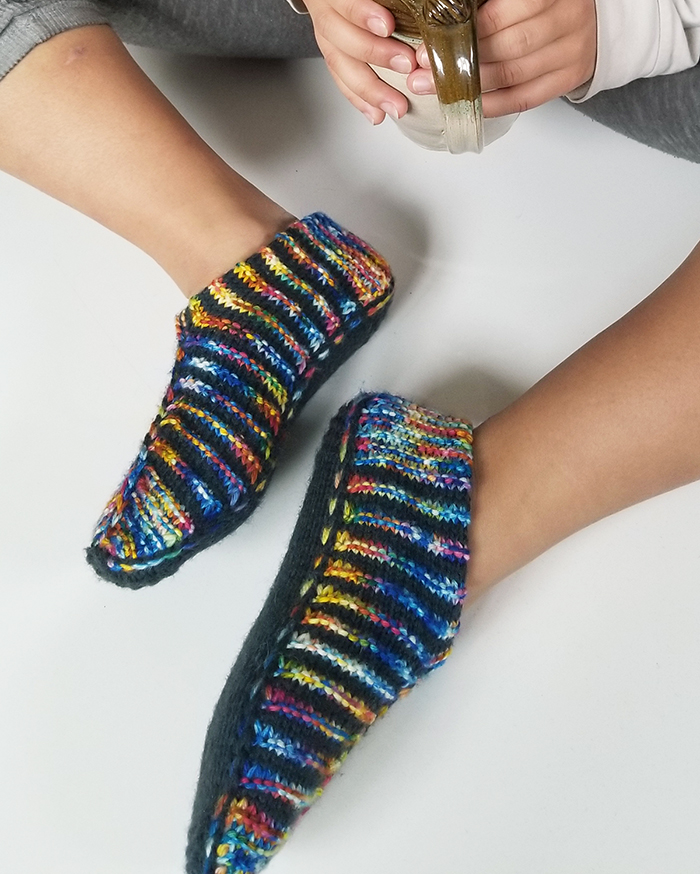
\includegraphics[width=\linewidth]{./photos/smallVersions/black_main_200dpi.jpg}

\subsection*{Pattern Key}

% formatting notes for charts and written directions

\vocab{Written instructions:} 

repeats = \longrepeat{thing to do}
%\vspace{-1em}

% abbreviation key - fill in with all abbreviations/stitch patterns used in design: written abbreviation, full stitch name or explanation
% try to keep them in sequential order as they appear in the pattern, or in an order that builds upon previous definitions
% chart symbols included in separate keys attached to their respective charts
% stitches with explanations must first be BOLDED, followed by colon then explanation
\begin{center}
{\renewcommand{\arraystretch}{1.5}
\begin{tabular}{| C{0.2\linewidth}  p{0.6\linewidth} | }
\thickhline \rowcolor{shadecolor} 
\textbf{Written}	& \textbf{Description} \\ \thickhline
CO 	& cast on \\
BO 	& bind off \\
RS 	& right side \\
WS 	& wrong side \\
k	&  knit \\
p	& purl   \\
k2tog 	& knit 2 together \\
sl 	& slip st (stitch) purlwise \mbox{\emph{\small unless otherwise indicated}} \\ 
sl1 wyib & sl 1 st with yarn in back \\
sl1 wyif & sl 1 st with yarn in front \\
psso 	& pass slipped st over \\
kfb 	& knit front back \\
\hline
\end{tabular}
}
\end{center}
\end{multicols}
\end{titlingpage}

%%%%%%%%%%%%%%%%%%%%%%%%%%%%%%%%%%%%%%%%%%%%%%%%%%
% BEGIN INSTRUCTIONS
\section*{Part 1: Sole}

\begin{frnote}
These instructions are written for the specified foot length. Foot length adjustments will be italicized in each part of the pattern.
\end{frnote}

Using MC, CO 3 (5, 6, 8) sts using the long tail method (or your preferred method). Work Row 1 a total of 6 (10, 12, 16) times to increase to 9 (15, 18, 24) sts.

\rowDir{Row 1} Sl1 wyif, k to 2 sts from end, kfb, k1.

~\\
Work sole in stockinette st by repeating Rows 2 and 3 an odd number of times, until piece measures 3 (6, 8.5, 11.5) ” / 7.5 (15, 21.5, 29) cm from CO \adjustment{or until 0.75 (1.25, 1.25, 1.75) ” / 2 (3, 3, 4) cm short of the toe}. Approx 7 (19, 31, 43) repeats. End after a WS row.

\rowDir{Row 2 (RS)} Sl1 wyif, k to end.

\rowDir{Row 3 (WS)} Sl1 knitwise wyif, p to 1 st from end, k1.

~\\
Work Row 4 a total of 6 (10, 12, 16) times to decrease to 3 (5, 6, 8) sts. BO all sts and break yarn.

\rowDir{Row 4} Sl1 wyif, k to 3 sts from end, k2tog, k1.

% PART 2
\section*{Part 2: Right Instep}

With WS facing and beginning in the right-hand corner of BO edge, use CC to pick up and knit 2 (3, 3, 4) sts.

\begin{frdirection}
\hspace{-2em}\vocab{XS only}

\rowDir{Next RS row} kfb, sl1 wyib, pick up and knit 1 st in selvedge, psso.

\rowDir{Next WS row} sl1 wyif, kfb, k1.
\end{frdirection}

Repeat Rows 5 and 6 a total of 2 (5, 6, 8) times to increase to 8 (13, 15, 20) sts.

\rowDir{Row 5 (RS)} Sl1 wyif, k to 2 sts from end, kfb, sl1 wyib, pick up and knit 1 st in selvedge (see diagram \vocab{A}), psso.

\rowDir{Row 6 (WS)} Sl1 wyif, k to 2 sts from end, kfb, k1.

\begin{wrapfigure}{R}{0.25\linewidth}
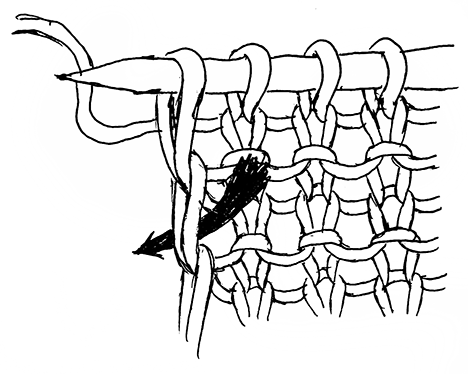
\includegraphics[width=\linewidth]{punk.png}
\emph{\small \textbf{A:} Insert R needle in this direction to pick up and knit in selvedge.}
\vspace{-1em}
\end{wrapfigure} \leavevmode

~\\
Join MC to work with both MC and CC in stripes. Repeat Rows 7-10 a total of 1 (4, 7, 10) times \adjustment{or until you are roughly at the halfway point of Part 1’s sole.} For a tighter fit at the ankle, work one or two extra repeats. When switching between colors, leave old color in front of RS, and pick up the new color from the left, twisting the two yarns.

\rowDir{Row 7 (RS, MC)} Sl1 wyif, k to 1 st from end, sl1 wyib, pick up and knit 1 st in selvedge, psso.

\rowDir{Row 8 (WS, MC)} Sl1 wyif, p to 1 st from end, k1.

\rowDir{Row 9 (RS, CC)} Sl1 wyif, k to 1 st from end, sl1 wyib, pick up and knit 1 st in selvedge, psso.

\rowDir{Row 10 (WS, CC)} Sl1 wyif, k to end.

~\\
Work Rows 7 and 8 once more. At the beginning of the next RS row and using the cable cast on, \longrepeat{CO 1 st in CC, CO 1 st in MC} until you have cast on 6 (8, 12, 14) additional sts for 14 (21, 27, 34) sts total.

~\\
Work Rows 9 and 10 once more. Repeat Rows 7-10 an additional 1 (4, 7, 10) times, then work Rows 7 and 8 once more. Break MC. Continue working only Rows 9 and 10 in CC until all selvedge sts along the heel have been worked. There should be 7 (13, 16, 22) garter ridges around heel. Do not break CC, as you will continue using it in Part 3.

% PART 3

\section*{Part 3: Left Instep}

Join MC. Repeat Rows 7-10 (reprinted below) 2 (5, 8, 11) more times.

\rowDir{Row 7 (RS, MC)} Sl1 wyif, k to 1 st from end, sl1 wyib, pick up and knit 1 st in selvedge, psso.

\rowDir{Row 8 (WS, MC)} Sl1 wyif, p to 1 st from end, k1.

\rowDir{Row 9 (RS, CC)} Sl1 wyif, k to 1 st from end, sl1 wyib, pick up and knit 1 st in selvedge, psso.

\rowDir{Row 10 (WS, CC)} Sl1 wyif, k to end.

~\\
Work Rows 7 and 8 once more, then break MC. Before starting the next RS row, hold the working needle WS together with the CO edge of Part 2 (WS faces WS). You will be working the CO sts together with the first 6 (8, 12, 14) live sts on the needle.

\begin{wrapfigure}{R}{0.3\linewidth}
\vspace{-2em}
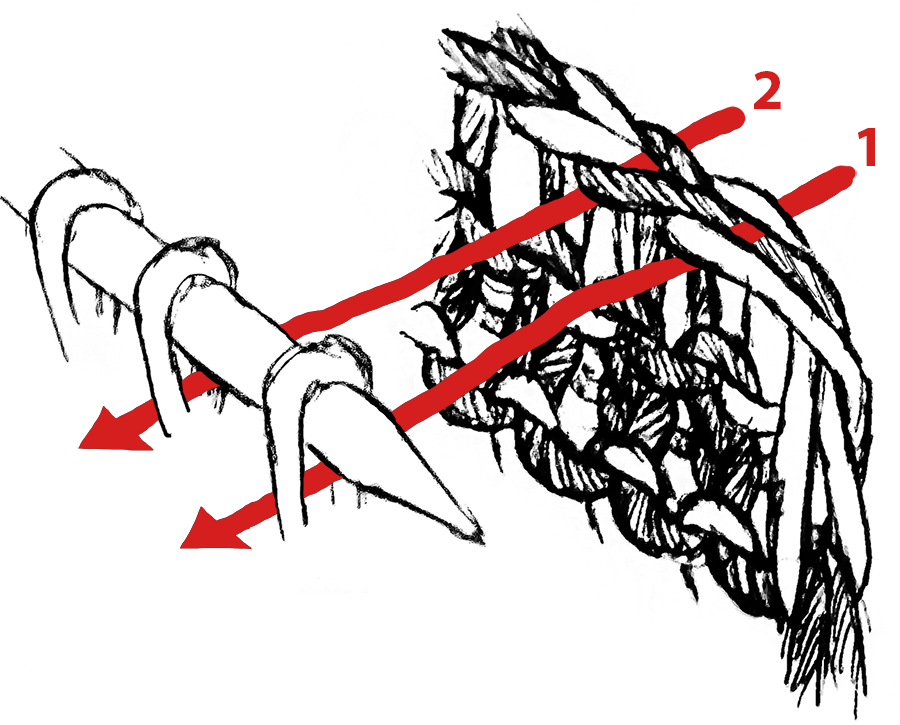
\includegraphics[width=\linewidth]{./diagrams/pickupCO.png}
\emph{\small \textbf{B:} Insert R needle along arrow \#1 to set up first p2tog. Arrow \#2 shows the next p2tog.}
\vspace{-1em}
\end{wrapfigure} \leavevmode

\rowDir{Next RS row (CC)}  Sl1 wyif. \repmark~ Insert needle into the right-hand corner of CO edge as if to purl, picking up both legs of the edge, then p2tog with next live st (see diagram \vocab{B}). Pass first st over second st to bind off one st. Repeat from \repmark, continuing to bind off until 8 (13, 15, 20) sts remain in total. K across the remaining sts to 1 st from end, sl1 wyib, pick up and knit 1 st in selvedge, psso.

\rowDir{Next WS row} Sl1 wyif, k to 1 st from end, sl1 wyif, pick up and purl 1 st in selvedge corner (see diagram \vocab{C}, make sure the selvedge st is in MC), psso.

\begin{wrapfigure}{R}{0.4\linewidth}
%\vspace{-1em}
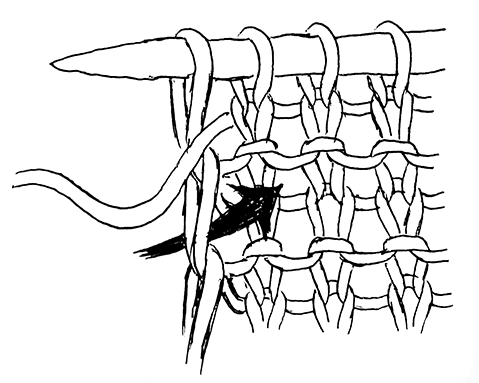
\includegraphics[width=\linewidth]{punp.png}
\emph{\small \textbf{C:} Insert R needle in this direction to pick up and purl in selvedge.}
\vspace{-1em}
\end{wrapfigure} \leavevmode

~\\
Rejoin MC. Work Rows 11-14 a total of 1 (4, 7, 10) times \emph{(or the same number of repeats as Part 2)} until you reach the toe.

\rowDir{Row 11 (RS, MC)} Sl1 wyib, k to 1 st from end, sl1 wyib, pick up and knit 1 st in selvedge, psso.

\rowDir{Row 12 (WS, MC)} Sl1 wyif, p to 1 st from end, sl1 wyif, pick up and purl 1 st in selvedge (selvedge st will be CC), psso.

\rowDir{Row 13 (RS, CC)} As Row 11.

\rowDir{Row 14 (WS, CC)} Sl1 wyif, k to 1 st from end, sl1 wyif, pick up and purl 1 st in selvedge (selvedge st will be MC), psso.

\vfill
\newpage
Break MC. Continuing in CC, work Rows 15-16 a total of 3 (5, 6, 8) times until you have 2 (3, 3, 4) sts remaining.

\rowDir{Row 15 (RS)} Sl1 wyib, k to 3 sts from end, k2tog, sl1 wyib, pick up and knit 1 st in selvedge, psso.

\rowDir{Row 16 (WS)} Sl1 wyif, k to 3 sts from end, k2tog, sl1 wyif, pick up and purl 1 st in selvedge (selvedge st will be CC), psso.

\begin{frdirection}
\hspace{-2em}\vocab{XS only}

\rowDir{Last RS row} Work Row 15 once more. 

\rowDir{Last WS row} k2tog, sl1 wyif, pick up and purl 1 st in selvedge, psso.
\end{frdirection}

Break yarn, leaving a 6”/15cm tail. Using the tail, sew the remaining sts to the front to close the toe. Repeat from Part 1 for second slipper.

%%%%%%%%%%%%%%%%%%%%%%%%%%%%%%%%%%%%%%%%%%%%%%%%%%
% APPENDICES (IF ANY)
\section*{Modification Suggestions}

\subsection*{High Arch/Instep Shaping}

\emph{This modification is shown in the yellow sample.} To add more room in the instep for high arches or deep heels, you can increase in Part 2 and then decrease in Part 3.

\subsubsection*{Part 2 Increases}

About an inch/2.5cm before the halfway point of Part 1's sole, begin increasing by replacing Rows 8 and 10 with the MC and CC Increase Rows, respectively. 

\rowDir{MC Increase Row (WS, MC)} Sl1 wyif, p to 2 sts from end, kfb, k1.

\rowDir{CC Increase Row (WS, CC)} Sl1 wyif, k to 2 sts from end, kfb, k1.

\subsubsection*{Part 3 Decreases}

\rowDir{MC Decrease Row (WS, MC)} Sl1 wyif, p to 3 sts from end, p2tog, sl1 wyif, pick up and purl 1 st in selvedge (selvedge st will be CC), psso.

\rowDir{CC Decrease row (WS, CC)} Sl1 wyif, k to 3 sts from end, k2tog, sl1 wyif, pick up and purl 1 st in selvedge (selvedge st will be MC), psso.

\vspace{-1em}
\begin{wrapfigure}{L}{0.3\linewidth}
\vspace{2em}
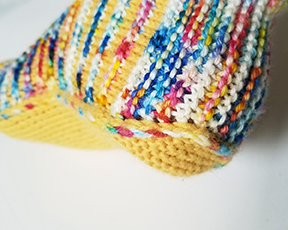
\includegraphics[width=\linewidth]{./photos/smallVersions/yellow_shapedheel.png}
\vspace{-4em}
\end{wrapfigure} \leavevmode

\subsection*{Heel Shaping}

\emph{This modification is shown in the yellow sample.} If your CC yarn is a superwash wool or other fiber that is not as bouncy as regular wool, the garter stitch heel may be prone to growing and falling down. Shaping the heel can bring up the back seam and reduce the stretchiness of the heel fabric.

~\\
In Part 2, in the first 3 (5, 6, 8) repeats of Rows 9 and 10, replace Row 9 with the Heel Decrease Row. Work Rows 9 and 10 as written 2 (3, 4, 6) more times. In the last 3 (5, 6, 8) repeats of Rows 9 and 10, replace Row 9 with the Heel Increase Row.

\rowDir{Heel Decrease Row (RS, CC)} Sl1 wyif, k to 3 sts from end, k2tog, sl1 wyib, pick up and knit 1 st in selvedge, psso.

\rowDir{Heel Increase Row (RS, CC)} Sl1 wyif, k to 2 sts from end, kfb, sl1 wyib, pick up and knit 1 st in selvedge, psso.

Alternatively (or in addition to this shaping), you can also substitute the garter stitch for a less elastic stitch, such as eye of partridge or half-linen stitch.

\vspace{-1em}
\begin{wrapfigure}{L}{0.3\linewidth}
\vspace{1em}
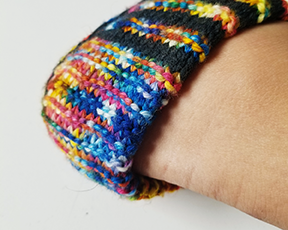
\includegraphics[width=\linewidth]{./photos/smallVersions/black_foldedcuff.png}
\vspace{-4em}
\end{wrapfigure} \leavevmode

\subsection*{Folded Cuff}

\emph{This modification is shown in the black sample.} Folding the cuff into the inside of the slipper not only changes the silhouette, but can also provide padding at the heel. Because the doubled fabric is also thicker and less elastic than the unfolded fabric, this modification might also help the slipper stay up.

~\\
After closing the toe, turn the slipper inside out and fold the back of the cuff so that the top edge meets the heel seam. Whipstitch the cuff edge to the middle of the heel's inside. The cuff should be secure even with just a few stitches.

\subsection*{Custom Sizing}

Making a custom size will start with creating a sole of the correct size and shape in Part 1. Perhaps you are creating a larger size than written for felting, or using a different gauge. These instructions assume that you know your desired foot width and foot length. You will also need your gauge in both stockinette and garter.

\begin{flushleft} \renewcommand{\arraystretch}{1.5}
\begin{tabular}{p{0.2\linewidth} p{0.75\linewidth}}
~ & \textbf{Foot width: \blank} \hspace{0.5in} \textbf{Foot length: \blank} \\ 
\textbf{Stitch gauge: \blank} & \textbf{Stockinette row gauge: \blank} \hspace{0.5in} \textbf{Garter row gauge: \blank} \vspace{1em} \\
\textbf{\mbox{1. Sole stitch} count: \blank} & Determine the full sole stitch count by dividing the desired foot width by your stitch gauge. \\
\textbf{\mbox{2. Sole CO count:} \blank} & Divide the sole stitch count by 3 (round up to nearest whole number). Make sure the difference between the sole stitch count and sole CO count is \emph{even}. \\
\textbf{\mbox{3. \# repeats of} \mbox{Row 1 and Row 4: \blank}} &  Subtract the sole CO count from the sole stitch count. \\
\textbf{\mbox{4. Wedge length:} \blank} & Get the length of the increase/decrease wedge pieces by dividing \#3 by your garter row gauge. \\
\textbf{\mbox{5. \# repeats of} \mbox{Rows 2 \& 3: \blank}} & Subtract two times \#4 from the desired foot length. Divide this result by your stockinette row gauge, and round up to the nearest odd number.
\end{tabular}\end{flushleft}

%%%%%%%%%%%%%%%%%%%%%%%%%%%%%%%%%%%%%%%%%%%%%%%%%%
% COPYRIGHT

\begin{frnote} \ssmall
Pattern and photographs \copyright 2020 Shanel Wu.
All rights reserved. In purchasing this pattern, you agree to print and use this pattern only for personal use. Do not redistribute or sell paper or electronic copies of this pattern.
\end{frnote}

\end{document}